\documentclass[12pt, a4paper]{article}
\usepackage[utf8]{inputenc}
\usepackage[T1]{fontenc}
\usepackage{color}
\usepackage{polski}
\usepackage{graphicx}
\usepackage{pdfpages}
\usepackage{indentfirst}
\usepackage{geometry}
\usepackage{setspace}
\usepackage{float}
\usepackage[backend=biber,style=numeric]{biblatex}

\addbibresource{bibliografia.bib}
\graphicspath{{./zdjecia/}}

\setstretch{1.5}

\geometry{
 a4paper,
 left=20mm,
 top=25mm,
 right=20mm,
 bottom=20mm
}

\begin{document}
\begin{sloppypar}
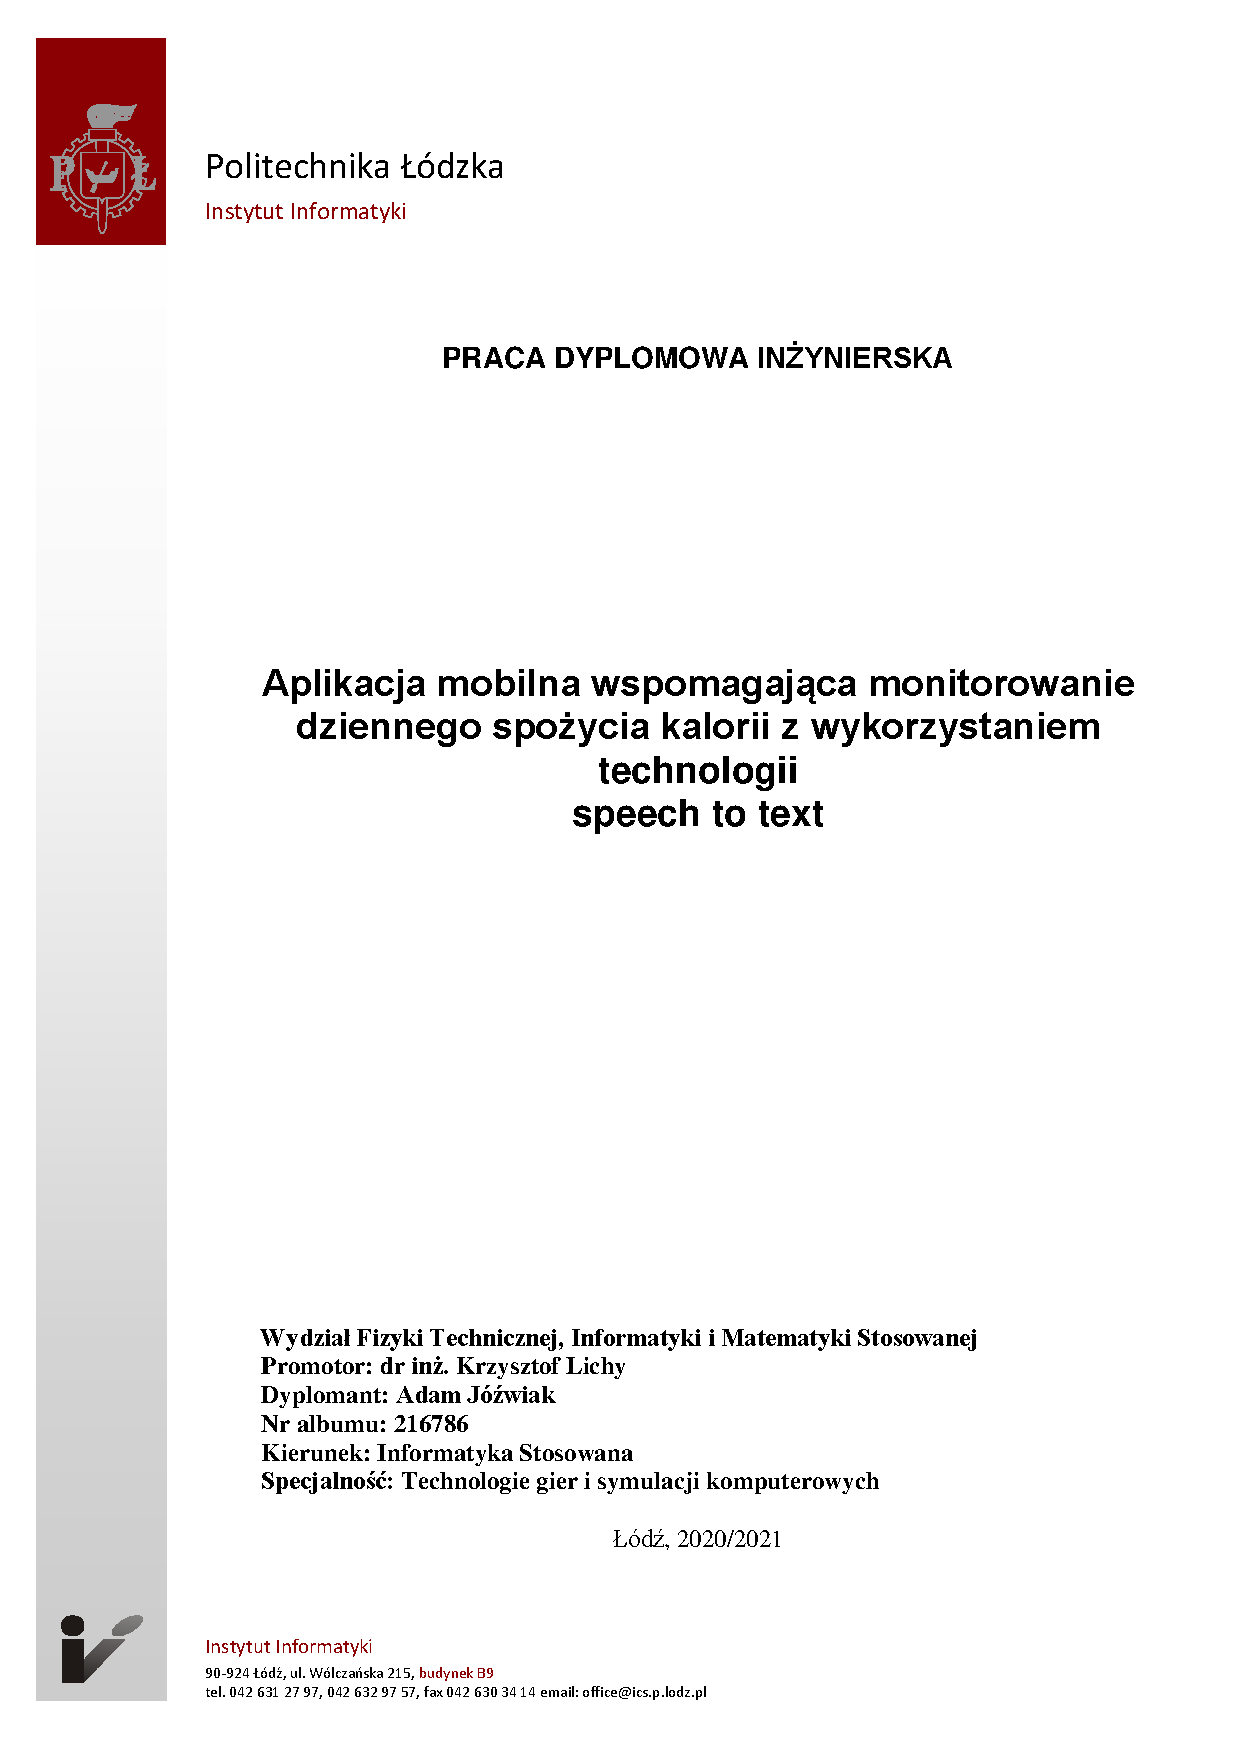
\includepdf{Strona_Tytulowa.pdf}

\tableofcontents
\newpage

\section{Wstęp}
{
  \subsection{Problematyka}
  {
    W epoce internetu XXI wieku, gdy wiedza jest narzędziem powszechnie dostępnym, a 
    każdy ma możliwość zdobycia informacji na interesujący go w mniejszym,
    lub większym stopniu temat, gdy media oraz tak zwani "influencerzy" promują zdrowy
    styl życia, popularnym trendem ostatnich lat staje się dbanie o własne ciało. 
    Trend popędzany również łatwym dostępem do najróżniejszych portali
    społecznościowych i chęcią pokazania Swoich zdjęć na forum publicznym sprawił, 
    że co roku znacznie zwiększa się ogólna ilość ludzi chętnych do uczęszczania na
    siłownię i odbywania regularnych treningów.
    \\ \\
    Równie ważną częścią dbania o Swoje ciało, oprócz treningów siłowych, jest 
    zastosowanie odpowiedniej diety. Nie jest to zadanie trywialne, ponieważ jest 
    ono w pełni zależne od zapotrzebowania osoby zainteresowanej, stąd istnienie
    zawodów takich jak "dietetyk". W związku z tym wiele osób zainteresowanych
    rozpoczęciem procesu odchudzania sięga po jedną z najprostszych i skutecznych
    metod, a mianowicie liczenie zjedzonych kalorii. Rekomendowana ilość
    dziennego ich spożycia jest zależna od bardzo dużego wachlarza czynników, 
    takich jak, przykładowo: płeć, wiek, wzrost, tryb życia, oraz wiele innych, 
    jednak w pracy naukowej zatytułowanej "How many calories should I eat a day?"
    \cite{cal}, autor podsumował, iż rekomendowaną dzienną ilością spożytych kalorii 
    dla przeciętnego mieszkańca Stanów Zjednoczonych, jest:
    \begin{itemize}
      \item mężczyzna - około 2500 kcal
      \item kobieta - około 2000 kcal
    \end{itemize}
    Bez odpowiedniego notowania procedura liczenia kalorii nie jest jednak efektywna, 
    stąd ludzie przyzwyczajeni do wygody oferowanej przez technologię, sięgają po 
    różnego rodzaju aplikacje, mające jeszcze bardziej ułatwić to, i tak już trywialne
    zadanie.

    Chodź na rynku istnieje już wiele aplikacji udostępniających taką funkcjonalność,
    używanie ich jest często zadaniem nieprzyjemnym i czasochłonnym, polegającym
    na wykonaniu całych serii kliknięć przeprowadzających użytkownika z jednego menu
    do drugiego, w celu wyszukania i dodania składników do listy spożytych artykułów,
    co długofalowo przekłada się na porzucenie chęci prowadzenia notatek dotyczących
    spożytych kalorii. 
    Brakuje na rynku rozwiązania, które udostępniłoby łatwy i szybki
    w użyciu interfejs, oraz w bardzo krótkim okresie czasowym pozwoliłoby wyszukać 
    i dodać interesujące użytkownika produkty. Dodatkowym atutem byłoby wzbogacenie
    takiej aplikacji o moduł wykorzystujący mowę ludzką, do jeszcze większego 
    usprawnienia całego procesu.
  }
  \subsection{Cel i zakres pracy}
  {
    Celem niniejszej pracy dyplomowej jest stworzenie aplikacji mobilnej, mającej 
    za zadanie wspomóc użytkownika w prowadzeniu notatek świadczących o dziennym
    spożyciu kalorii. Aplikacja udostępniać będzie moduł speech to text,
    który w jeszcze większym stopniu ułatwi proces wyszukiwania produktów, a całość
    będzie uporządkowana w postaci przejrzystego i prostego w obsłudze interfejsu
    graficznego.

    Praca obejmuje implementację logiki przy użyciu języka programowania \emph{Dart},
    natomiast wygląd aplikacji, oraz interakcje pomiędzy poszczególnymi modułami
    zarządzane są przy pomocy frameworku \emph{Flutter}.

    \color{red} ???????????????
  }
  %\subsection{Keywords}
  %{

  %}
}

\section{Teoria}
{
  \subsection{Rynek aplikacji mobilnych}
  {
    Urządzenia mobilne są obok komputerów uważane za jedne z najbardziej rewolucyjnych
    i przełomowych technologii opracowanych w XX wieku. I chodź pierwsze prototypy 
    powstawały już wcześniej niż lata czterdzieste, nie przypominały w obsłudze urządzeń
    dostępnych dzisiaj i wykorzystywane były głównie w celach militarnych.
    Oficjalnie za pierwszy telefon w historii uważany jest egzemplarz Motorola 
    DynaTAC 8000x, wynaleziony przez Martina Coopera, pracującego wtedy dla firmy 
    Motorola \cite{history1}. I chodź zamienienie prototypu na urządzenie dostępne
    komercyjnie zajęło następną dekadę, tak relatywnie ciężkie początki telefonów
    zamieniły się w prawdziwą lawinę nowych rozwiązań. Chodź nie jest to wiedza
    powszechna, tak pierwszy smartphone powstał już w 1994 roku, a był to IBM's Simon
    \cite{history2}. Tak więc przez następne lata firmy prześcigały się technologicznie,
    każda przyczyniając się w mniejszym lub większym stopniu do rozwoju rynku urządzeń
    mobilnych, aż do 2007 roku, niosącego wydarzenie znane powszechnie jako jedno 
    z najważniejszych w historii telefonów komórkowych. Rok w którym Steve Jobs 
    zaprezentował na konferencji MacWorld 2007 pierwszy model smartphone'a iPhone 2G,
    który w pełni pozbył się przycisków na rzecz dotykowego ekranu. Moment ten wyznaczył
    tor po jakim aż po dziś dzień poruszają się wszystkie firmy zajmujące się tworzeniem
    urządzeń mobilnych i w ten sposób oficjalnie rozpoczęła się era smartphone'ów.

    Początkowo wszelkie aplikacje mobilne były dostarczane głównie przez producentów
    telefonów i były one "wbudowane" - nie istniała możliwość zainstalowania
    ich po zakupie produktu. W roku 1983 Steve Jobs planował już jednak stworzenie
    miejsca, w którym oprogramowanie mogłoby być kupowane przy użyciu linii
    telefonicznych \cite{history4}. Tak oto w 2008 roku została uruchomiona usługa
    "App Store", wraz z flotą 500 dostępnych aplikacji. Jednak Apple jest firmą
    restrykcyjną i tworzenie nowych aplikacji na system operacyjny iOS nie było 
    zadaniem trywialnym. Na szczęście codziennego użytkownika i ogólnego rozwoju, 
    iOS nie posiadał monopolu na aplikacje mobilne, ponieważ w 2005 roku Google
    wykupiło firmę, której flagowy produkt jest bardzo dobrze pod nazwą Android OS
    \cite{history3}.

    Android jest to system operacyjny oparty na rodzinie systemów Linux, co bezpośrednio
    przełożyło się na jego darmowość i pozwoliło szturmem podbić świat, jak można
    zaobserwować na raporcie przygotowanym przez firmę StatCounter \cite{os}.
    \begin{figure}[H]
      \centering
      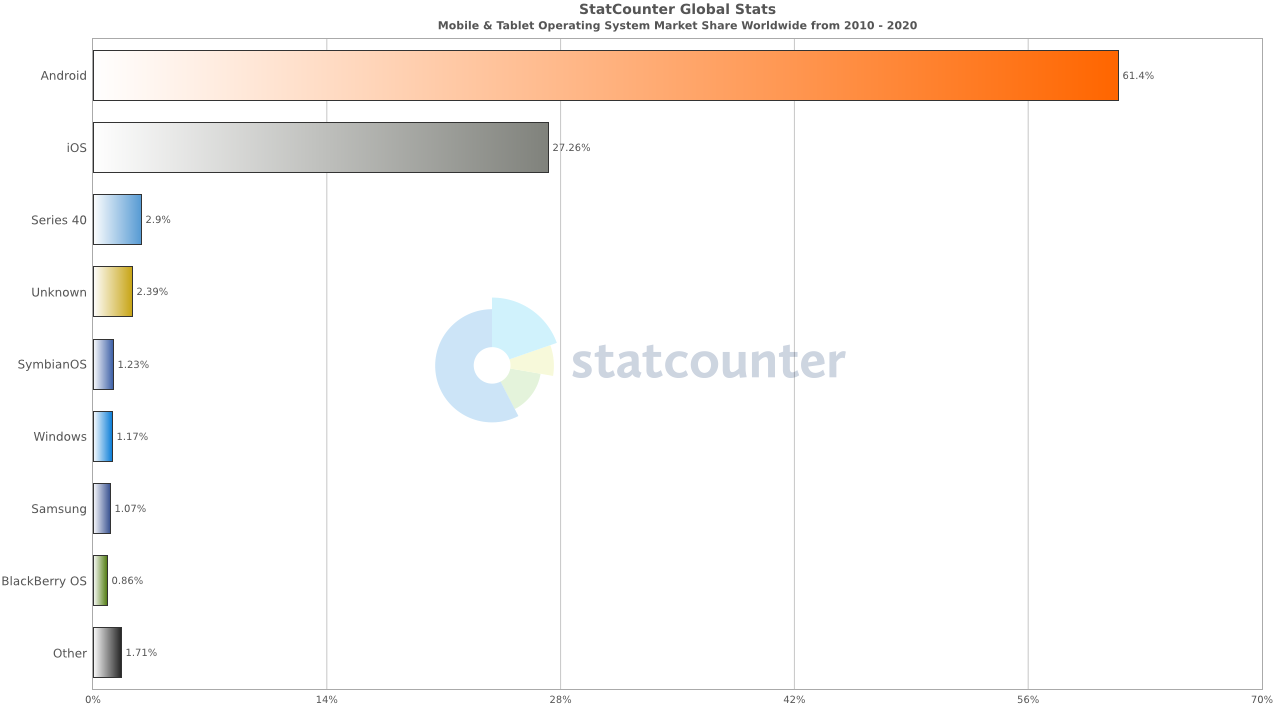
\includegraphics[width=0.9\textwidth]{android_chart.png}
      \caption{Wykres udziału w rynku poszczególnych mobilnych systemów operacyjnych na przestrzeni 12 lat}
      \label{fig:android}
    \end{figure}
    Łatwa dostępność, ilość urządzeń na których jest on zainstalowany, szeroki wachlarz
    możliwości - te cechy napędzały ambicje twórców aplikacji mobilnych. Zaoferowany
    przez firmę Google Play Store, w przeciwieństwie do App Store pozwala na darmowe
    udostępnienie produktów o ile spełniają one odpowiednie warunki.

    Wraz z tak prężnym rozwojem rynku smartphone'ów, rozpoczęła się zmiana trendów.
    I o ile od początku XXI wieku światem królowały komputery, oferujące cały zasób 
    możliwości od nauki, po rozrywkę, tak smartphony z roku na rok coraz bardziej 
    zaczęły przypominać swoich stacjonarnych braci. 
    \begin{figure}[H]
      \centering
      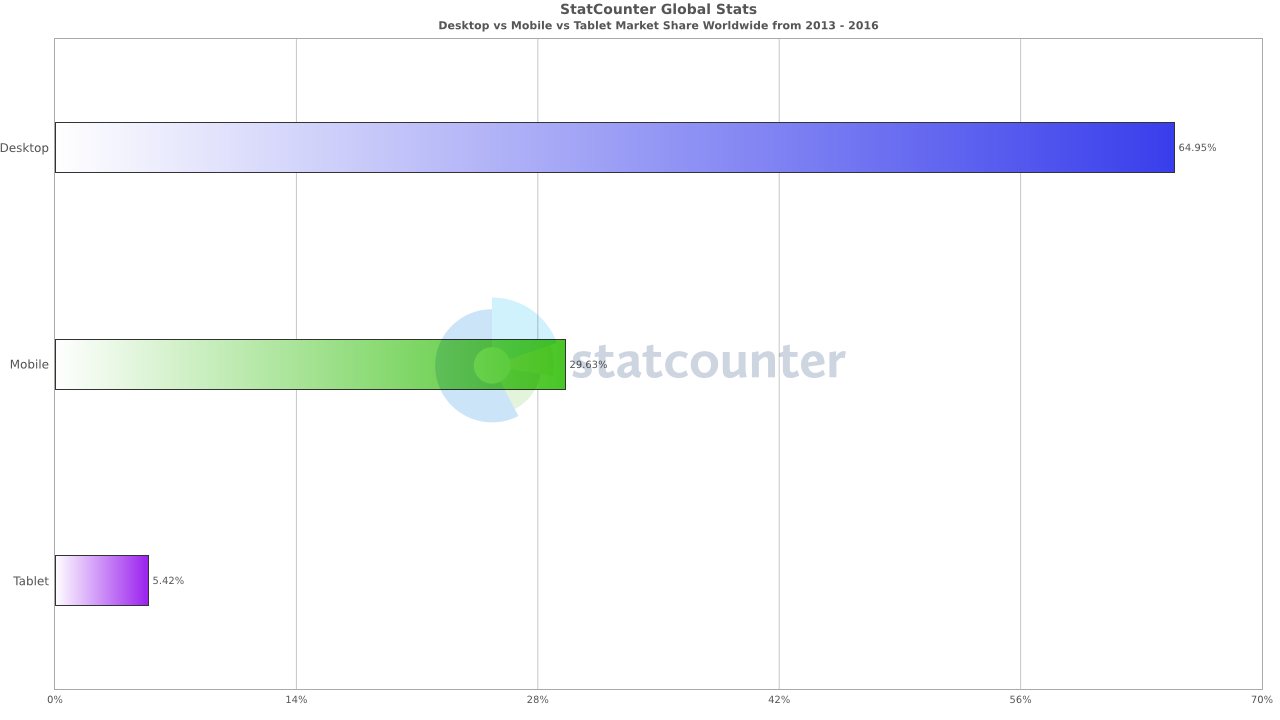
\includegraphics[width=0.9\textwidth]{systems_chart1.png}
      \caption{Komputery, a smartphony na przestrzeni lat 2013-2016}
      \label{fig:2013}
    \end{figure} 
    \begin{figure}[H]
      \centering
      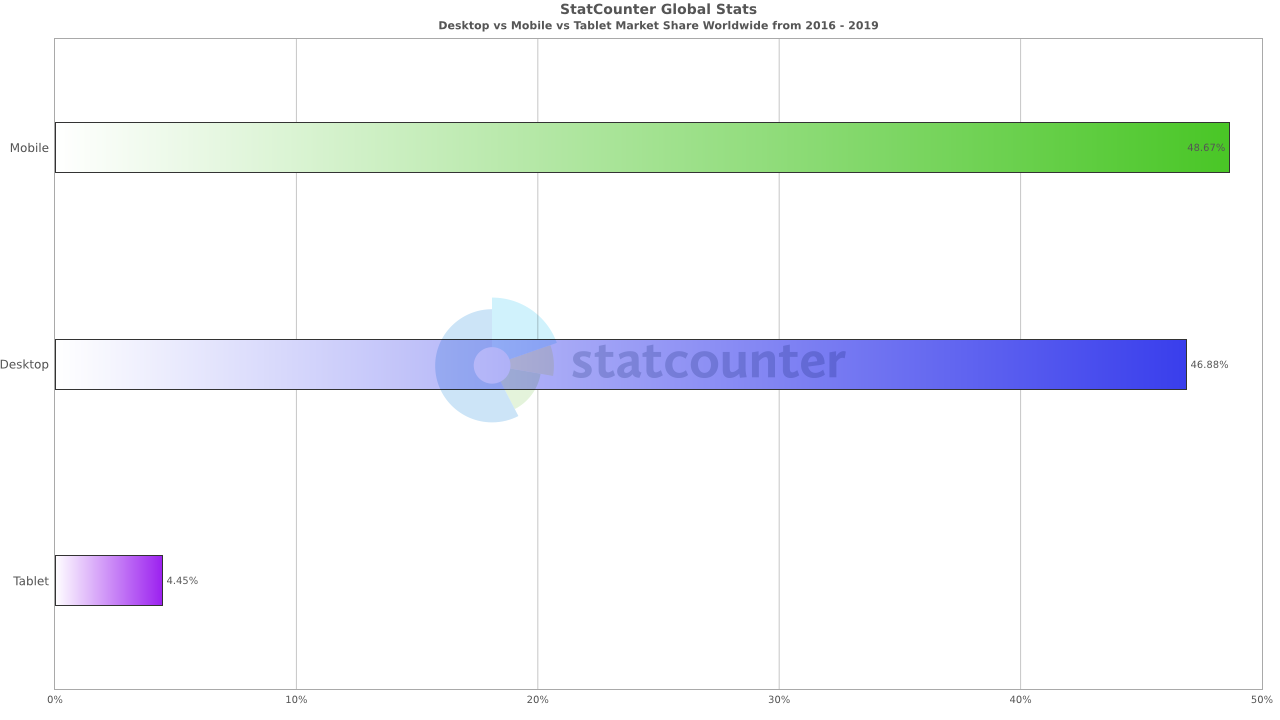
\includegraphics[width=0.9\textwidth]{systems_chart2.png}
      \caption{Komputery, a smartphony na przestrzeni lat 2016-2019}
      \label{fig:2016}
    \end{figure} 
    Jednak urządzenia mobilne były i są w stanie zaoferować dużą większą wygodę 
    użytkowania, przenośność, oraz system znacznie łatwiejszy do przyswojenia dla 
    przeciętnego człowieka, nie wymagający szczególnej wiedzy do poprawnego
    zarządzania. Stąd u młodzieży umiejętności obsługi komputerów stacjonarnych
    zaczęła zanikać, jako że przestaje ona być tak kluczowa jak była jeszcze 10 lat
    temu. Jak podaje strona Broadbandsearch \cite{dvm}, już w 2016 roku większość "ruchu"
    internetowego była spowodowana przez urządzenia mobilne, bo aż 51.3\%, i po 
    rok 2021 oscyluje stabilnie w granicach 52\%. Jak podaje ten sam portal,
    różnice pomiędzy rokiem 2013, a 2019 w ilości czasu spędzanego dziennie na 
    użytkowaniu smartphonów i desktopów wygląda następująco:
    \begin{itemize}
      \item Średni czas użytkowania komputerów/laptopów spadł ze 144 minut dziennie, do 128 minut
      \item Średni czas użytkowania urządzeń mobilnych wzrósł z 88 minut, do średnio 203 minut dziennie 
    \end{itemize} 
    Takie wyniki sprawiły, że coraz więcej firm musiało zacząć liczyć się z 
    rynkiem urządzeń mobilnych, a obecnie częstą praktyką przy tworzeniu aplikacji 
    przeznaczonych zarówno na komputery stacjonarne, jak i smartphony, lub przy 
    pisaniu stron internetowych, jest stylizowanie ich najpierw na mniejsze ekrany,
    a następnie dostosowywanie pod urządzenia desktopowe. W przypadku marketingu, 
    zamiast "optymalizować" go pod kątem urządzeń mobilnych, zaczęto tworzyć zupełnie
    oddzielne kampanie marketingowe zarówno dla desktopów jak i smartphone'ów
    \cite{mobile_strategy}.
  }
  \subsection{Programowanie aplikacji na urządzenia mobilne}
  {
    
  }
  \subsection{Speech to text}
  {
    Popularną opinią jest, iż lenistwo idzie w parze z ludzkim rozwojem 
    technologicznym. Wiele przypadków potwierdza tą regułę, sam Bill Gates, założyciel
    firmy Microsoft powiedział:\\ 
    “I choose a lazy person to do a hard job. 
    Because a lazy person will find an easy way to do it.”
    W duchu tych słów, ludzie jako rasa mają w zwyczaju być leniwymi, dlatego
    naturalną rzeczą stał się fakt, iż pisanie na klawiaturze nie jest najbardziej 
    optymalną techniką "porozumiewania się" z maszynami.
    
    W roku 1952, Bell Laboratories stworzyło system "Audrey", który był w stanie 
    rozpoznać wypowiedziane pojedyńcze cyfry, a 10 lat później, "Shoebox" od IBM
    mógł zrozumieć i odpowiedzieć na 16 słówek w języku Angielskim \cite{speech_history}.
    W latach siedemdziesiątych XX wieku, Amerykański Departament Obrony rozpoczął
    projekt o nazwie "SUR" - The Speech Understanding Research, którego owocem
    był "Harpy", system będący w stanie rozpoznać 1000 słów. Współzawodnictwo wielu
    firm w zakresie rozpoznawania mowy doprowadzało do powstawania dużej ilości nowych
    modeli, oraz metod, jeszcze bardziej optymalizujących cały proces.

    Do roku 2001, estymowana dokładność systemów rozpoznawania mowy wynosiła około 80\%,
    i przez dłuższy nie zostały osiągnięte godne uwagi postępy. Sytuacja jednak
    zmieniła się dzięki firmie Google, która uaktywniła w roku 2012 usługę Google 
    Voice Search. Okazała się ona być ogromnym sukcesem, jako że była to darmowa 
    aplikacja dostępna na urządzeniach mobilnych, stąd dzięki jej szerokiej dostępności,
    firma miała okazję zebrać dane pochodzące od milionów użytkowników, co przełożyło
    się bezpośrednio na poprawę dokładności algorytmu. Z czasem kolejne firmy
    zaczęły inwestować w technologię, a okres od roku 2010 do 2020 jest uważany za
    szczególnie ważny dla historii technologii rozpoznawania mowy. Tak oto w roku 2021
    użytkownicy mają dostęp do:
    \begin{itemize}
      \item Google Voice Search / Google Assistant - Google 
      \item Siri - Apple
      \item Cortana - Microsoft
      \item Alexa - Amazon
      \item I wiele innych ...
    \end{itemize}
    Firmy te prześcigają się o tytuł dokładności rozpoznawania mowy. W roku 2016, IBM
    osiągnęło wartość błędu 6,9\%. W 2017, Microsoft udało się osiągnąć błąd o
    wartości 5,9\%, jednak IBM szybko kontratakowało swoim 5,5\%. Firmy te
    nadal pozostają w tyle przy Google, którego błąd w 2017 roku osiągnął 4,9\% i do
    dziś pozostaje najdokładniejszym systemem rozpoznawania mowy dostępnym na rynku.
    Wraz z upływem czasu, technologia ta stawać się będzie coraz szybsza i
    efektywniejsza i bardzo możliwe jest, iż stanie się ona głównym interfejsem służącym
    komunikacji pomiędzy człowiekiem, a maszyną. 

    Przez większą część historii technologii "Speech Recognition", 
    najpopularniejszą metodą był HMM - "Hidden Markov Model" \cite{markov_article},
    opracowany już w latach osiemdziesiątych. W dużym skrócie, zamiast używania 
    słów i szukania w nich dźwiękowego wzorca, ma on za zadanie przewidzieć
    prawdopodobieństwo tego, że nieznane dźwięki mogą być słowami.\\   
    Proces analizy rozpoczyna się od zebrania informacji dźwiękowej,
    zwykle przy użyciu mikrofonu, i już na tym stadium pojawiają się pierwsze 
    problemy, takie jak:
    \begin{itemize}
      \item wyłapanie odpowiednich słów spośród dźwięków tła - szumu samochodów na 
      ulicy, lub inne osoby rozmawiające w bliskiej odległości.
      \item w przypadku szybko mówiącego rozmówcy, rozróżnienie w którym momencie
      wypowiedzi słowa kończą się, oraz kiedy zaczynają się kolejne.
      \item rozróżnianie różnych akcentów i sposobów mówienia pojedynczych jednostek,
      na przykład to samo zdanie wypowiedziane przez 10 letnią dziewczynkę, brzmieć
      będzie zupełnie inaczej, wypowiedziane przez 70 letniego mężczyznę. 
      \item odróżnianie homofonów - słów wymawianych w ten sam sposób, ale mających
      inne znaczenie
      \item poprawne zinterpretowanie zdań brzmiących w bardzo podobny sposób, ale
      oznaczających zupełnie różne rzeczy
    \end{itemize} 
    Dodatkowo, różne języki mają różną gramatyczną strukturę, co dodatkowo utrudnia
    stworzenie zunifikowanego systemu, zdolnego do przetwarzania wielu języków w 
    podobny sposób.\\
    Kolejnym krokiem jest przetworzenie zebranych danych na spektogram przy użyciu
    Szybkiej Transformaty Fouriera \cite{fourier}, oraz rozszczepienie
    rezultatu na mniejsze części, które poddawane są analizie mającej na celu
    określenie w jakich momentach znajdują się słowa. Następnie każde z nich są
    porównywane pod względem fonetycznego brzmienia i w ten sposób program stara
    się przewidzieć dokładne słowo, wypowiedziane przez użytkownika.

    W dzisiejszych czasach, technologia rozpoznawania mowy w głównej mierze opiera
    się na algorytmach sztucznej inteligencji połączonych z HMM.
  }
  \subsection{Bazy danych i ich rodzaje}
  {

  }
  \subsection{Chmurowe bazy danych}
  {

  }
  \subsection{API}
  {

  }
  \subsection{Analiza konkurencyjnych rozwiązań}
  {

  }
  \subsection{Wymagania funkcjonalne}
  {

  }
  \subsection{Wymagania niefunkcjonalne}
  {

  }
}

\section{Technologie i narzędzia wykorzystane w projekcie}
{
  \subsection{Flutter}
  {

  }
  \subsection{Dart}
  {

  }
  \subsection{Cloud Firestore}
  {

  }
  \subsection{Android Studio}
  {

  }
  \subsection{Android Emulator}
  {

  }
  \subsection{VIM}
  {

  }
}

\section{Proces powstawania aplikacji}
{
}

\section{Podsumowanie}
{
}

\section{Indeks rysunków}

\section{Bibliografia}
{
  \printbibliography
  %https://www.oracle.com/pl/database/what-is-database/#link5
  %https://smartbees.pl/blog/co-jest-api-wszystko-o-interfejsie-programowania-aplikacji
  %https://www.cdc.gov/nchs/products/databriefs/db360.htm
  %https://runrepeat.com/gym-membership-statistics
  %https://fs.siteor.com/ecdl/files/RODZAJE_BAZ_DANYCH_I_ICH_BUDOWA.pdf?1289369360
}

\end{sloppypar}
\end{document}